\section{Librer\'ia de An\'alisis de Conceptos Formales}

\textbf{Introducci\'on}

Toda la teor\'ia que se va a desarrollar a lo largo de este punto est\'a extra\'ida del libro de Ganter.
\textcolor{red}{A\~nadir referencia libro Ganter. Pedir datos a Angel}

El an\'alisis de conceptos formales es un entorno conceptual que estructura, analiza y visualiza conocimiento a partir de datos proporcionados 
como una relaci\'on binaria entre objetos y atributos.

Como se ha explicado anteriormente, un contexto formal \( (G, M, I) \) consiste en dos conjuntos, G y M, y una relaci\'on binaria \( I \subseteq G \times M \). Los elementos 
de G se llaman objetos, los de M, atributos de \( (G, M, I) \). Si \(g \in G ~ y ~ m \in M \) est\'an relacionados seg\'un I, se escribir\'a 
\( (g,m) \in I ~ o ~ g I m \) y se leer\'a como ``el objeto g tiene el atributo m".

Para trabajar con contextos se utilizan varias funciones que se van a desgranar una a una en los siguientes puntos:

    \subsection{Leer concepto}

        \textbf{Descripci\'on}

        Como primera funci\'on se tiene la de obtener un concepto formal con su estructura adecuada teniendo la informaci\'on en un fichero. A la 
        hora de utilizar esta funci\'on se pueden usar ficheros xls, txt o r, ya que el resultado ser\'a el mismo, una variable de tipo data.frame 
        con toda la informaci\'on del fichero de entrada.
        \\

        \clearpage

        \textbf{C\'odigo}

        \lstinputlisting{r_code/FCA/read.fc.R}
        \bigskip

        \textbf{Ejemplo}

        Se va a proponer un ejemplo en el que se leer\'a de un fichero txt que contiene lo siguiente:

        \begin{verbatim}
            1 2 3 4 5
            Compose Even ODD
            0 0 1
            0 1 0
            0 0 1
            1 1 0
            0 0 1
        \end{verbatim}

        \begin{figure}[H]
            \centering
            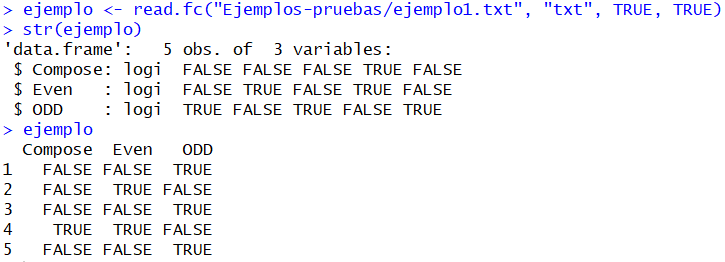
\includegraphics{readfc}
            \caption{Ejemplo de leer de fichero un concepto formal}
            \label{fig:readfc}
        \end{figure}

        Como se puede observar en la imagen de arriba, lo primero que se ejecuta es la funci\'on \textbf{read.fc}, que tal y como se ha comentado 
        antes, es la encargada de leer el fichero. A continuaci\'on, se extrae el formato de la variable en la que se ha guardado la 
        salida de la funci\'on que se est\'a probando, y se observa, que tal y como se esperaba es un data.frame.

        Por \'ultimo, vemos que en la variable ejemplo se ha guardado la informaci\'on que se ten\'ia en el archivo txt.

    \subsection{Operador de derivaci\'on de atributos a objetos}

        \textbf{Descripci\'on}

        Dado un contexto formal \( (G, M, I) \), se llama operador de derivaci\'on de atributos a objetos a la 
        funci\'on \( ^\uparrow : 2^G \rightarrow 2^M \)

        \[ A^\uparrow = { m \in M | <g,m> \in I ~ para ~ todo ~ g \in A } \]

        El conjunto \( A^\uparrow \) es el de los atributos compartidos por todos los objetos de A, es decir, este operador devolver\'a 
        un conjunto de atributos que ser\'an los que contiene un determinado objeto.
        \\
        
        \clearpage

        \textbf{C\'odigo}

        \lstinputlisting{r_code/FCA/mp.R}


        \textbf{Ejemplo}

        Para los ejemplos de este apartado y los tres siguientes, se va a usar un mismo contexto que se generar\'a de forma aleatoria:

        Comencemos generado dicho contexto:

        \begin{figure}[H]
            \centering
            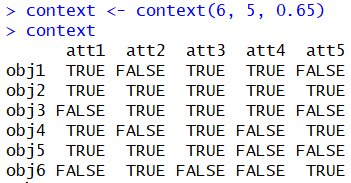
\includegraphics{mp1}
            \caption{Generaci\'on de contexto a usar}
            \label{fig:mp1}
        \end{figure}


        A partir de ese contexto, se aplica la funci\'on de derivaci\'on de atributos a objetos. Le pasamos el contexto y el atributo 4, y 
        como podemos observar en la salida, obtenemos los objetos 1, 2 y 3.

        \begin{figure}[H]
            \centering
            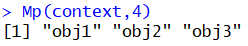
\includegraphics{mpej}
            \caption{Ejemplo de derivaci\'on de atributos a objetos}
            \label{fig:mpej}
        \end{figure}


    \subsection{Operador de derivaci\'on de objetos a atributos}

        \textbf{Descripci\'on}

        Dado un contexto formal \( (G, M, I) \), se llama operador de derivaci\'on de objetos a atributos a la 
        funci\'on \( ^\downarrow : 2^M \rightarrow 2^G \)

        \[ B^\downarrow = { g \in G | <g,m> \in I ~ para ~ todo ~ m \in B } \]

        El conjunto \( B^\downarrow \) es el de los objetos compartidos por todos los atributos de B, en este caso, este operador devolver\'a 
        un conjunto de objetos que ser\'an los que contiene un determinado atributo.
        \\


        \textbf{C\'odigo}

        \lstinputlisting{r_code/FCA/gp.R}

        \clearpage

        \textbf{Ejemplo}

        Comenzamos recordando cu\'al es el contexto que se va a usar:

        \begin{figure}[H]
            \centering
            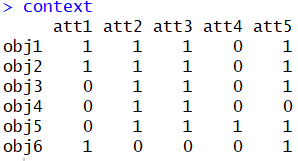
\includegraphics{context}
            \caption{Contexto que se va a usar}
            \label{fig:context}
        \end{figure}

        A continuaci\'on, se aplica la funci\'on de derivaci\'on de objetos a atributos. Le pasamos el contexto y en este caso, el objeto 4, y 
        como podemos observar en la salida, obtenemos los atributos 2 y 3.

        \begin{figure}[H]
            \centering
            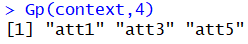
\includegraphics{gpej}
            \caption{Ejemplo de derivaci\'on de objetos a atributos}
            \label{fig:gpej}
        \end{figure}


    \subsection{Operador de doble derivaci\'on de atributos a objetos}

        \textbf{Descripci\'on}

        El conjunto que devuelve el operador \( A^\uparrow \) tambi\'en se suele representar como \( A' \), por lo que en este caso, 
        el operador de doble derivaci\'on de atributos a objetos se representar\'a como \( A'' \).


        \[ A'' = (A^\uparrow)^\downarrow \]

        Es decir, al conjunto que se obtiene como salida del operador de derivaci\'on de atributos a objetos, se le aplica el operador 
        de derivaci\'on de objetos a atributos.


        \clearpage

        \textbf{C\'odigo}

        \lstinputlisting{r_code/FCA/mp2.R}

        \bigskip

        \textbf{Ejemplo}

        Usando el mismo contexto que en los anteriores, se aplica el operador de doble derivaci\'on de atributos a objetos a dicho 
        contexto y al objeto4, de nuevo.

        Y obtenemos como resultado los atributos 3 y 4.

        \begin{figure}[H]
            \centering
            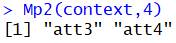
\includegraphics{mp2ej}
            \caption{Ejemplo de doble derivaci\'on de atributos a objetos}
            \label{fig:mp2ej}
        \end{figure}



    \subsection{Operador de doble derivaci\'on de objetos a atributos}

        \textbf{Descripci\'on}

        El conjunto que devuelve el operador \( B^\downarrow \) tambi\'en se suele representar como \( B' \), por lo que en este caso, 
        el operador de doble derivaci\'on de objetos a atributos se representar\'a como \( B'' \).


        \[ B'' = (B^\downarrow)^\uparrow \]

        Es decir, al conjunto que se obtiene como salida del operador de derivaci\'on de objetos a atributos, se le aplica el operador 
        de derivaci\'on de atributos a objetos.

        \clearpage

        \textbf{C\'odigo}

        \lstinputlisting{r_code/FCA/gp2.R}

        \bigskip

        \textbf{Ejemplo}

        Por \'ultima vez, se usa el mismo contexto que en los anteriores, se aplica el operador de doble derivaci\'on de 
        objetos a atributos al contexto y al atributo4 para terminar de observar el comportamiento de los cuatro operadores.

        Y obtenemos como resultado los objetos 2 y 4.

        \begin{figure}[H]
            \centering
            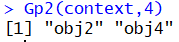
\includegraphics{gp2ej}
            \caption{Ejemplo de doble derivaci\'on de objetos a atributos}
            \label{fig:gp2ej}
        \end{figure}



    \subsection{Concepto formal}

    
        \textbf{Descripci\'on}

        Dado un contexto formal \( K = (G, M, I) \), se dice que un par \( <A,B> \) es un 
        concepto formal de \(K\) si \( A^\uparrow = B ~ y ~ B^\downarrow = A\), donde \( A \subseteq G ~ y ~ B \subseteq M \).
        
        Es decir, \( <A,B> \) ser\'a un concepto formal si A contiene exactamente todos los objetos que comparten los atributos de B, y a su 
        vez, B contiene exactamente todos los atributos que comparten los objetos de A.
        \\

        \clearpage

        \textbf{C\'odigo}

        \lstinputlisting{r_code/FCA/is.formal.concept.R}

        \bigskip

        \textbf{Ejemplo}

        Para este ejemplo, se va utilizar el contexto creado en el anterior ejemplo y el concepto del siguiente fichero excel:

        \begin{figure}[H]
            \centering
            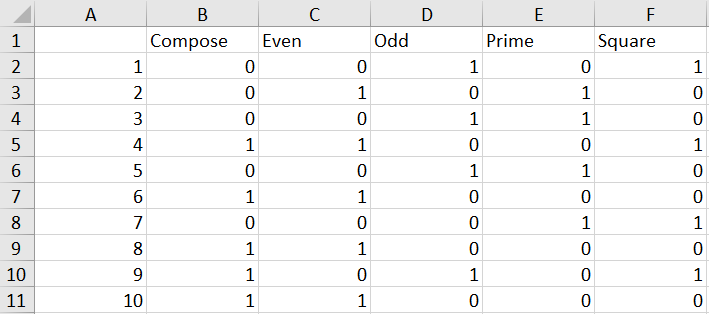
\includegraphics{excel}
            \caption{Contexto}
            \label{fig:excel}
        \end{figure}


        Con los dos elementos anteriores, se va a ejecutar la funci\'on para ver si efectivamente es un concepto formal del contexto o no:

        \begin{figure}[H]
            \centering
            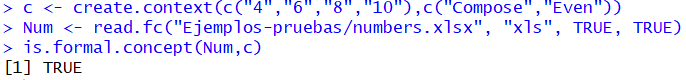
\includegraphics{isformal}
            \caption{Ejemplo de contexto formal}
            \label{fig:isformal}
        \end{figure}

        \clearpage



    \subsection{Crear concepto}

        \textbf{Descripci\'on}

        En esta librer\'ia, un concepto consta de una lista con dos vectores diferentes. Luego, con esta funci\'on, se puede crear un concepto 
        pas\'andole como par\'ametros dos vectores diferentes.
        Cada uno de dichos vectores, tendr\'a como nombre g y m en este orden, y representar\'an los objetos y atributos.
        \\
        

        \textbf{C\'odigo}

        \lstinputlisting{r_code/FCA/create.context.R}

        \bigskip

        \textbf{Ejemplo}

        \begin{figure}[H]
            \centering
            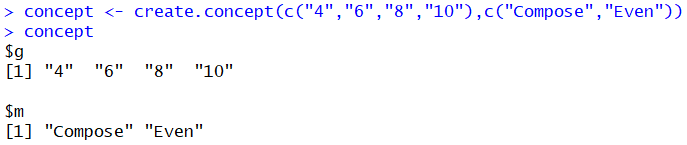
\includegraphics{createContext}
            \caption{Ejemplo de crear concepto}
            \label{fig:createContext}
        \end{figure}




    \subsection{Supremo}


        \textbf{Introducci\'on}
    
        En este caso, se a comenzar con unas definiciones necesarias para los dos pr\'oximos puntos.
        \\

        Dado un contexto formal \( K = (G, M, I) \), se llama ret\'iculo de conceptos de \(K\), y se denota por \( B (K) \), al ret\'iculo 
        formado por los conceptos con la relaci\'on de orden:

        \( (A_{1}, B_{1}) \leq (A_{2}, B_{2}) ~ si ~ y ~ solo ~ si ~ A_{1} \subseteq A_{2} \)
        \( o ~ equivalentemente, ~ B_{1} \supseteq B_{2} \)

        \bigskip


        El orden establecido entre los conceptos formales indica cu\'al de ellos es m\'as espec\'ifico. Luego,  \( (A_{1}, B_{1}) \leq (A_{2}, B_{2})\) 
        quiere decir que  \( (A_{1}, B_{1}) \) es m\'as espec\'ifico que \( (A_{2}, B_{2}) \) denomin\'andose subconcepto o, igualmente, que  
        \( (A_{2}, B_{2}) \) es m\'as general denomin\'andose superconcepto.

        \bigskip


        \textbf{Descripci\'on}

        Siendo \((A_{1}, B_{1}) \) y \((A_{2}, B_{2})\) dos conceptos formales de un contexto formal, se define el supremo como:

        El superconcepto com\'un m\'as peque\~no de \((A_{1}, B_{1}) \) y \((A_{2}, B_{2})\):

        \[ (A_{1}, B_{1}) \vee (A_{2}, B_{2}) = ((A_{1} \cup A_{2})'', ~ B_{1}\cap B_{2}) \]

        \bigskip
        \textbf{C\'odigo}

        En este caso, se han desarrollado dos funciones diferentes. Una que obtiene el supremo de dos conceptos:

        \lstinputlisting{r_code/FCA/supremum.R}

        Y otra, que de un conjunto de conceptos, obtiene su supremo:

        \lstinputlisting{r_code/FCA/supremum.set.fc.R}

        \clearpage

        \textbf{Ejemplo}

        En este ejemplo, se realiza el supremo entre dos conceptos:

        \begin{figure}[H]
            \centering
            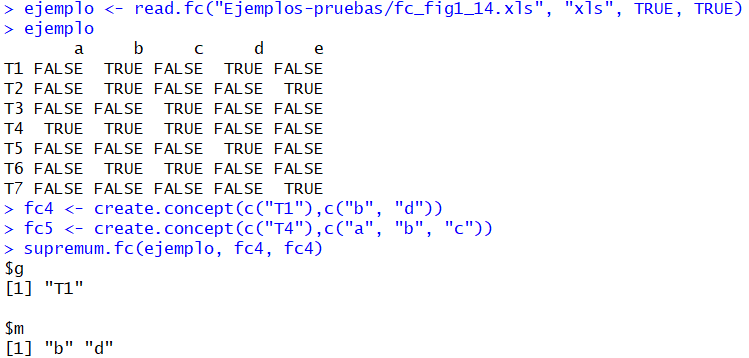
\includegraphics{supremum}
            \caption{Ejemplo de supremo de dos conceptos}
            \label{fig:supremum}
        \end{figure}


    \subsection{\'Infimo}

    
        \textbf{Descripci\'on}

        Siendo \((A_{1}, B_{1}) ~ y ~ (A_{2}, B_{2})\) dos conceptos formales de un contexto formal, se define el \'infimo como:

        El subconcepto com\'un m\'as grande de \((A_{1}, B_{1}) ~ y ~ (A_{2}, B_{2})\):

        \[ (A_{1}, B_{1}) \wedge (A_{2}, B_{2}) = (A_{1} \cap A_{2}'', ~ (B_{1}\cup B_{2})'') \]

        \clearpage

        \textbf{C\'odigo}

        En este caso, tambi\'en tenemos dos funciones. El \'infimo de dos conceptos:

        \lstinputlisting{r_code/FCA/infimum.R}

        Y otra, que de un conjunto de conceptos, obtiene su \'infimo:

        \lstinputlisting{r_code/FCA/infimum.set.fc.R}

        \bigskip

        \textbf{Ejemplo}

        Este ejemplo corresponde con la primera funci\'on, en la que se calcula el \'infimo de dos conceptos:

        \begin{figure}[H]
            \centering
            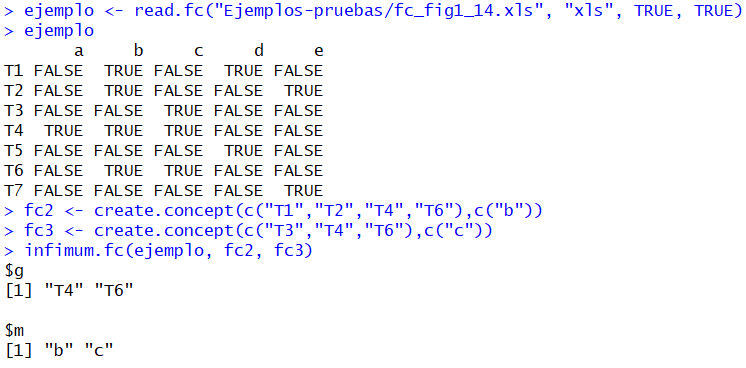
\includegraphics{infimum}
            \caption{Ejemplo de \'infimo de dos conceptos}
            \label{fig:infimum}
        \end{figure}



    \subsection{Objeto concepto}

    
        \textbf{Descripci\'on}

        Siendo \( (G, M, I) \) un contexto formal. Entonces para cada objeto \( g \in G\), el correspondiente objeto concepto es:

        \[ \gamma g:=(\{g\}'', \{g\}') \]

        Es decir, para esta funci\'on se utiliza un contexto y un objeto, y nos devuelve un nuevo concepto siguiendo la definici\'on 
        anterior.
        \\

        \clearpage

        \textbf{C\'odigo}

        Se han realizado dos funciones diferentes. En esta primera se calcula el objeto concepto para un solo objeto:
        
        \lstinputlisting{r_code/FCA/object.concept.fc.R}

        Y la segunda, calcula todos los objetos conceptos del contexto:
        \lstinputlisting{r_code/FCA/all.object.concept.R}

        \bigskip

        \textbf{Ejemplo}

        En este ejemplo, se genera un contexto aleatorio y se calcula el objeto concepto del objeto 4:

        \begin{figure}[H]
            \centering
            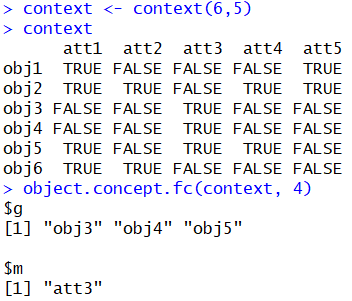
\includegraphics{objcon}
            \caption{Ejemplo de objeto concepto}
            \label{fig:objcon}
        \end{figure}




    \subsection{Atributo concepto}

    
        \textbf{Descripci\'on}

        Siendo \( (G, M, I) \) un contexto formal. Entonces para cada atributo \( m \in M\), el correspondiente atributo concepto es:

        \[ \mu m:=(\{m\}'', \{m\}') \]

        Es este caso, para esta funci\'on se utiliza un contexto y un atributo, y nos devuelve un nuevo concepto siguiendo la definici\'on 
        anterior.
        \\


        \textbf{C\'odigo}

        De nuevo, se divide en dos funciones. Esta calcula el atributo concepto para un solo atributo:

        \lstinputlisting{r_code/FCA/attribute.concept.fc.R}

        Y esta segunda, calcula todos los atributos conceptos del contexto:
        \lstinputlisting{r_code/FCA/all.attribute.concept.fc.R}

        \clearpage

        \textbf{Ejemplo}

        En este caso usamos el mismo contexto que en el anterior:

        \begin{figure}[H]
            \centering
            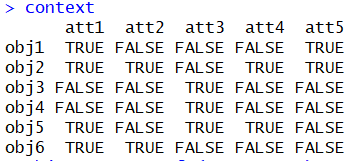
\includegraphics{conconcepto}
            \caption{Contexto para el ejemplo}
            \label{fig:conconcepto}
        \end{figure}

        Y calculamos el atributo concepto del atributo 4:

        \begin{figure}[H]
            \centering
            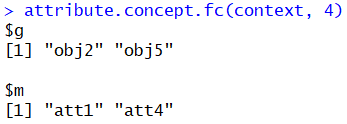
\includegraphics{attcon}
            \caption{Ejemplo de atributo concepto}
            \label{fig:attcon}
        \end{figure}



    \subsection{Todos los objetos conceptos y atributos conceptos}
       
        
        \textbf{Descripci\'on}

        Por \'ultimo, con esta funci\'on se podr\'an obtener todos los conceptos formales de un contexto.
        \\


        \textbf{C\'odigo}

        \lstinputlisting{r_code/FCA/all.fc.R}

        \bigskip

        \textbf{Ejemplo}

        Se genera un contexto aleatorio con un n\'umero peque\~no de objetos y atributos.

        \begin{figure}[H]
            \centering
            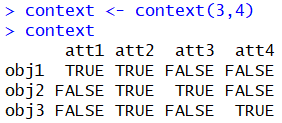
\includegraphics{contextoAll}
            \caption{Contexto a usar en el ejemplo siguiente}
            \label{fig:contextoAll}
        \end{figure}
        
        \bigskip
        Y se generan todos los conceptos formales:


        \begin{figure}[H]
            \centering
            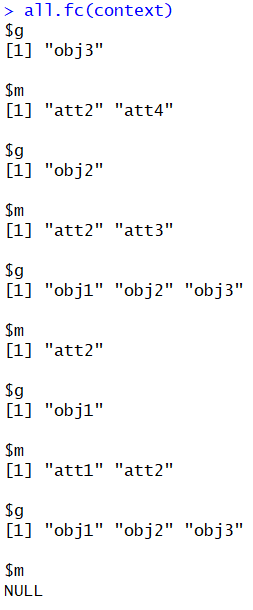
\includegraphics{allcontext}
            \caption{Ejemplo de todos los conceptos formales de un contexto}
            \label{fig:allcontext}
        \end{figure}

        \clearpage



\subsection{Next closure}

        \textbf{Descripci\'on}
    
    
        \textbf{C\'odigo}
    
    
        \textbf{Ejemplo}


        
\subsection{Generadores minimales}


    \textbf{Introducci\'on}

    Aunque seg\'un el anteproyecto este algoritmo se deber\'ia encontrar en la parte de mi compa\~nero, se ha decidido pasar este algoritmo 
    a esta parte porque pertenece al campo de FCA, aunque podr\'ia aplicarse en otros muchos.

    \textcolor{red}{Con esta explicaci\'on basta?}

    Este algoritmo y sus respectivas funciones se han desarrollado a partir de un art\'iculo publicado por el tutor de 
    TFG y su grupo de investigaci\'on\cite{cla2012}.
    Se va a comenzar con algunas definiciones para que se conozca el contexto:

    Una base implicacional \(K\) se define como un conjunto \(\mathcal{L}\) de implicaciones de \(K\) desde el cual, mediante las reglas de 
    Armstrong puede ser deducida cualquier implicaci\'on v\'alida de \(K\). El objetivo es obtener una base implicacional de tama\~no 
    m\'inimo.

    Aunque el algoritmo del cierre se explicar\'a detalladamente en el segundo vol\'umen de este TFG en grupo, se a\~nade aqu\'i su 
    definici\'on, ya que se usar\'a en este algoritmo de generadores minimales:

    Siendo \(\Gamma\) un conjunto de implicaciones y \(A\) un conjunto de atributos. El cierre de \(A\) en la l\'ogica de \(SL_{FD}\) se define como 
    el m\'aximo conjunto de atributos \(A^+\) como \(\Gamma \vdash A \rightarrow A^+\).


    \bigskip
    \textbf{Descripci\'on}

    En este punto, se van a calcular el conjunto de generadores minimales de un conjunto de implicaciones. Este algoritmo funciona aplicando 
    el algoritmo \(SL_{FD}Closure\) al conjunto de conjuntos de implicaciones.

    La entrada de este algoritmo consta de un conjunto de atributos \(M\) y un conjunto de implicaciones \(\Gamma\) sobre los atributos en \(M\).
    La salida ser\'a el conjunto de conjuntos cerrados dotados con todos los generadores que lo generan.

    \[
        {\langle C, mg(C) \rangle : C ~ is ~ a ~ closed ~ set ~ of ~ attributes}    
    \]

    \[
        where ~ mg(C) = {D: ~ D ~ is ~ a ~ mingen ~ and ~ D^+ = C}    
    \]

    Esto se puede ver como el ret\'iculo de conceptos en el que se han agregado etiquetas con el generador minimal a cada conjunto cerrado.
    Con esta idea, se van a necesitar operadores que nos permitan trabajar con estos tipos de conjuntos. Es decir, conjuntos de pares 
    \( \langle A, B \rangle \), tales que \( A \subseteq M\) es un intent y \( B \subseteq 2^M\) cumple las siguientes condiciones:

    1. \(X \subseteq A ~ for ~ all ~ X \in B\).

    2. \(X,Y \in B ~ and ~ X \subseteq Y ~ imply ~ X = Y\)

    Este tipo de conjuntos son llamados Labeled Set of Intents (LSI). Dados dos LSIs \(\Phi\) y \(\Psi\), se define la uni\'on de ambos como 
    el m\'inimo LSI que satisfaga:
    \\
    - Si \( \langle A_{1}, B_{1} \rangle \in \Phi \) y \(A_{1} \neq A_{2} \) para todo \( \langle A_{2}, B_{2} \rangle \in \Psi \) 
    entonces \( \langle A_{1}, B_{1} \rangle \in \Phi \sqcup \Psi \)
    \\
    - Si \( \langle A_{1}, B_{1} \rangle \in \Psi \) y \(A_{1} \neq A_{2} \) para todo \( \langle A_{2}, B_{2} \rangle \in \Phi \) 
    entonces \( \langle A_{1}, B_{1} \rangle \in \Phi \sqcup \Psi \)
    \\
    - Si \( \langle A, B_{1} \rangle \in \Psi \) y \( \langle A, B_{1} \rangle \in \Phi \) entonces \( \langle A, B_{3} \rangle \in \Phi \sqcup \Psi \) 
    siendo \(B_{3}\) el conjunto de los elementos minimales de \(B_{1} \cup B_{2}\)

    
    A continuaci\'on se va a definir un nuevo operador, el trivial, que dado un \(M\) y \(\Gamma\) devuelve el siguiente LSI:


    \[
        trv(M, \Gamma) = {\langle X, {X} \rangle: X \subseteq M ~ con ~ A \not \subseteq X ~ para ~ todo ~ A \rightarrow B \in \Gamma} )    
    \]

    Tambi\'en se va a necesitar una forma para a\~nadir un par a un LSI, que se define como:

    \[
        Add(\langle C, {D} \rangle, \Phi) = {\langle A \cup C, ~ {X \cup D: X \in B} \rangle : \langle A, B\rangle \in \Phi}    
    \]


    Por \'ultimo, se a especificar el pseudoc\'odigo de este algoritmo, del cual se ha partido para daserrollarlo en R para este TFG:
    \bigskip

    \IncMargin{1em}
\begin{algorithm}[H]
    \SetKwFunction{MinGen}
    \SetAlgoLined
    % \LinesNumbered
    \DontPrintSemicolon
    \SetKw{KwOr}{or}
    \KwIn{  
        $M,$
        $\Gamma$
    }
    \KwOut{
        $\Phi$
    }
    \Begin{
        \If{ $ \Gamma = \emptyset $ } {
            \ $ \Phi = trv(M, \Gamma) $\;
        } \Else {
            \ $ \Phi = trv(M, \Gamma) $\;
             \ForEach{$ A \rightarrow B \in \Gamma $}{
                \ $ (A^+, \Gamma ') = Cls(A, \Gamma) $\;
                \ $ \Phi = \Phi \sqcup Add( \langle A^+, \{A\} \rangle, MinGen(M \backslash A^+, \Gamma ') ) $\;
             }
            }
            
        \Return $ \Phi $
    }%end beginre
    \caption{MinGen algorithm}
    \label{alg:1}
\end{algorithm}
\DecMargin{1em}

    \bigskip
    \textbf{C\'odigo}

    Aunque a lo largo de este algoritmo se utilizan diversas funciones, aqu\'i se van a incluir las m\'as importantes.
    
    Se comienza con el principal, el algoritmo MinGen al que est\'a dedicado este punto:

    \lstinputlisting{r_code/FCA/mingen.R}

    A continuaci\'on, una de las m\'as importantes, la funci\'on trv:

    \lstinputlisting{r_code/FCA/trv.R}

    Y, por supuesto, la funci\'on add, que se ha explicado con anterioridad:

    \lstinputlisting{r_code/FCA/add.R}

    \bigskip
    \textbf{Ejemplo}

    Para el ejemplo de este algoritmo, se ha usado un conjunto de tres implicaciones, formadas por cuatro elementos diferentes.
    La salida del algoritmo es un conjunto de cinco pares, tal y como se puede ver en la siguiente imagen:

    \begin{figure}[H]
        \centering
        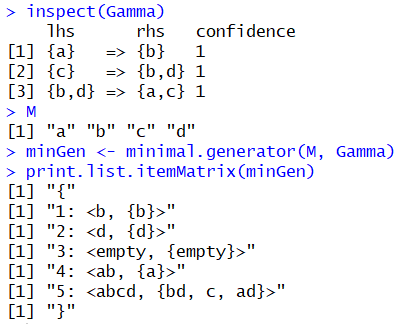
\includegraphics{minGen}
        \caption{Ejemplo de generadores minimales}
        \label{fig:minGen}
    \end{figure}

    

    \bigskip
    \textbf{Comparativa/Versiones}

    La versi\'on original de la funci\'on trv se ha mejorado implementando una poda para no recorrer todos los subconjuntos, y as\'i 
    mejorar el tiempo del algoritmo general.

    A continuaci\'on se puede ver una comparativa de tiempos entre las dos versiones. Se puede observar la versi\'on original sin la poda, y 
    la segunda en la que se aplica dicha mejora. La versi\'on que se ha incluido en esta memoria corresponde a la segunda, ya que 
    realiza la poda.

    \begin{figure}[H]
        \centering
        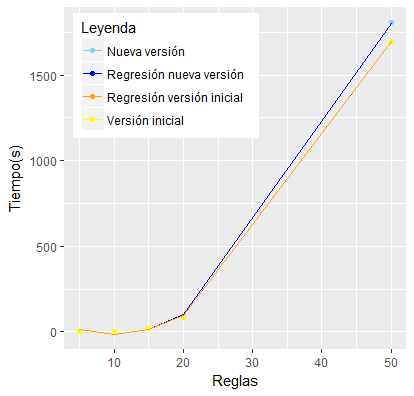
\includegraphics{tiemposMinGen}
        \caption{Gr\'afica de tiempos}
        \label{fig:tiemposMinGen}
    \end{figure}


    Los par\'ametros de entrada para realizar las pruebas de tiempo de este algoritmo se han realizado con el generador aleatorio definido en 
    el punto anterior, generando de esta manera conjuntos de implicaciones de diferentes tama\~nos.

